\subsubsection{Environment}

The task environment is a virtual graphical computer program for building virtual block structures using either a Leap Motion or keyboard and mouse. 

\begin{figure}[H]
\centering
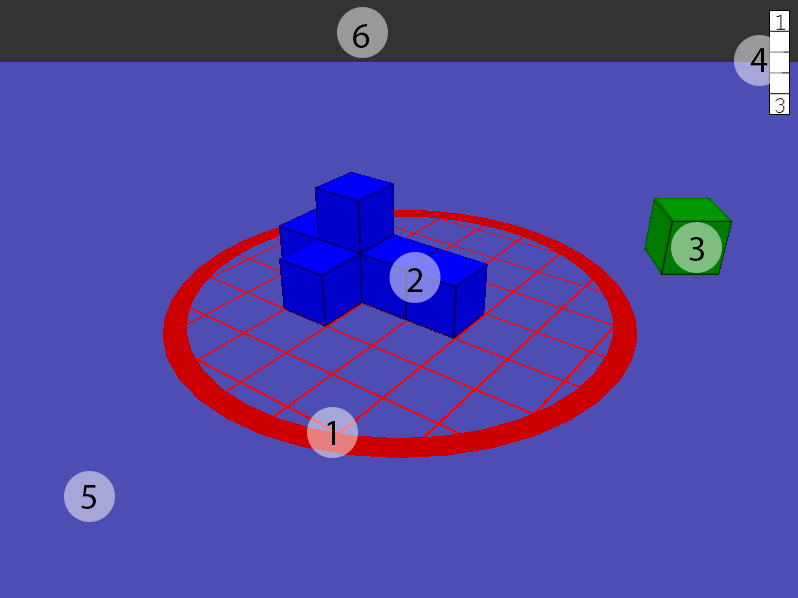
\includegraphics[width=\textwidth]{env_comps}
\caption{\label{fig:environmentcomps} Common rendering of the task environment. Visual elements: 1) Circular grid 2) Building blocks 3) Creation block 4) Target indicator 5) Floor 6) Horizon}
\end{figure}

\noindent Figure~\ref{fig:environmentcomps} shows a common rendering from the task environment where all groups of visual elements have been labeled. In the center of the screen users are presented with a circular grid that is segmented into several squares, effectively representing a grid with an circular border. On this grid building blocks can be positioned, either directly on the grid or stacked on top of other building blocks. New building blocks can be obtained by interacting (clicking with the mouse or grabbing with the Leap Motion) with the creation block outside the circular grid. The target indicator on the top right corner gives the user a representation of the block structure that should be created on the grid before the user can move further.

% Circular grid
% Creation block
% Building blocks
% Floor
% Horizon
% Target indication

\textbf{Design rationale}
The program was developed with the use of jMonkeyEngine, an open source 3D game engine written in Java. For development we used the Software Development Kit that comes with the engine, which provides a high level interface for numerous 3D functions and data-structures (e.g. spatial manipulation, quaternions and 3D meshes) and also provides a high degree of control for developers by being completely compatible with the Java programming language. 

Both the User Interface (UI) and the user interactions were designed to be minimalistic, simple and intuitive in order to prevent users having to learn a lot before they could use the system. 


\textbf{Does it work?}